%% ##############################################################################################################
%  This dissertation template is a modification of the Bj\"orn Brandenburg template
%  The old template is available here: https://www.cs.unc.edu/~bbb/
%  Some minor adjustments were made to account for the inexplicable rule changes of UNC since 2013
%  You are free to use these template files, but do not use any of the included example figures.
%    S Reece Boston, April 2022
%% ##############################################################################################################

\chapter{The Newtonian Theory of Stellar Pulsations\label{ch:chapter2}}

\section{Introduction}\label{sec:chapter2:intro}
\lipsum[1]

\section{Stellar hydrodynamics}\label{sec:chapter2:hydro}
\lipsum[2]
\lipsum[3][1-2]
\begin{subequations} \label{eq:chapter2:static1}
\begin{align} 
	\nabla^2\Phi &= 4\pi G\rho\label{eq:chapter2:static1A}\\
	\del{\rho}{t} &= 0\\
	\nabla P &= -\rho\nabla\Phi\label{eq:chapter2:euler}.
\end{align}
\end{subequations}
\lipsum[3][3-4]


\section{Simple stellar models}\label{sec:chapter2:stellar}
\lipsum[6]

\subsection{The uniform-density star}\label{subsec:chapter2:uniform}
\lipsum[7]

\subsection{Polytropic fluid spheres}\label{subsec:chapter2:polytrope}
\lipsum[9][1-5]
It can be shown that \equref{newtonian:static1} reduces to the Lane-Emden equation \citep{Lane1870}
\begin{equation}\label{eq:chapter2:laneemden}
	\frac{1}{\xi^2} \dif{}{\xi}\left( \xi^2 \dif{\theta}{\xi}\right) = -\theta^n.
\end{equation}
\lipsum[10][2-3]
\begin{subequations}\label{eq:chapter2:laneemdenExact}
\begin{align}
	n = 0, &\qquad \theta = 1 - \frac{\xi^2}{6}\\
	n = 1, &\qquad \theta = \frac{\sin \xi}{\xi}\\
	n = 5, &\qquad \theta = \frac{1}{\sqrt{1 + \xi^2/3}}.
\end{align}
\end{subequations}
\lipsum[10][4]


\section{Newtonian stellar pulsation code}\label{sec:chapter2:code}


\subsection{Exact error measures}\label{subsec:chapter2:code1}
\lipsum[1][3-8]
This is shown in \figref{chapter2:polyexact}.  See also \figref{chapter2:polyresid}.  \lipsum[2][11].

\begin{figure*}
	\resizebox{\linewidth}{!}{\input{./chapter2/graphs/exact_all_10K}}
	\caption[Error in Lane-Emden polytrope code]{
	The error from comparing numerical solutions to Lane-Emden \equref{chapter2:laneemden} to the exact polytrope solution of \equref{chapter2:laneemdenExact}.
	\label{fig:chapter2:polyexact}}
\end{figure*}

\subsection{Internal error measures}\label{subsec:chapter2:code2}

In addition, I can convert the solution in terms of 
$\xi,\theta$ to \equref{newtonian:laneemden}  to a solution in terms of physical variables such as $r, \rho, P, \Phi$ and insert 
these variables back into the original equations \equref{newtonian:static1} to calculate a scaled residual, \eg for 
\equref{newtonian:static1A},
\begin{equation}\label{eq:Residual}
 \mathrm{res}(r) = \frac{\abs{ \dif{}{r}(r^2\dif{\Phi}{r})  - 4\pi G \rho r^2  }}
 		{\abs{\dif{}{r}(r^2\dif{\Phi}{r})}+\abs{4\pi G\rho r^2}}.
\end{equation}
Across a range of indices $n$, and for $N_{star}=10^5$, I find this residual to be less than or on the order of $10^{-12}$.
We define a root-mean square residual (RMSR)
\begin{equation}\label{eq:RMSR}
	\text{RMSR} = \sqrt{\frac{1}{\Rstar}\int_0^\Rstar \text{res}^2(r) dr}
\end{equation}
which gives an estimate of numerical error.  Graphs showing the above fraction for several polytropes are in Figures \ref{fig:chapter2:scalepolyexact}, \ref{fig:chapter2:scalepolyresid}.

\begin{figure*}
	\resizebox{\linewidth}{!}{% GNUPLOT: LaTeX picture with Postscript
\begingroup
  \makeatletter
  \providecommand\color[2][]{%
    \GenericError{(gnuplot) \space\space\space\@spaces}{%
      Package color not loaded in conjunction with
      terminal option `colourtext'%
    }{See the gnuplot documentation for explanation.%
    }{Either use 'blacktext' in gnuplot or load the package
      color.sty in LaTeX.}%
    \renewcommand\color[2][]{}%
  }%
  \providecommand\includegraphics[2][]{%
    \GenericError{(gnuplot) \space\space\space\@spaces}{%
      Package graphicx or graphics not loaded%
    }{See the gnuplot documentation for explanation.%
    }{The gnuplot epslatex terminal needs graphicx.sty or graphics.sty.}%
    \renewcommand\includegraphics[2][]{}%
  }%
  \providecommand\rotatebox[2]{#2}%
  \@ifundefined{ifGPcolor}{%
    \newif\ifGPcolor
    \GPcolorfalse
  }{}%
  \@ifundefined{ifGPblacktext}{%
    \newif\ifGPblacktext
    \GPblacktexttrue
  }{}%
  % define a \g@addto@macro without @ in the name:
  \let\gplgaddtomacro\g@addto@macro
  % define empty templates for all commands taking text:
  \gdef\gplbacktext{}%
  \gdef\gplfronttext{}%
  \makeatother
  \ifGPblacktext
    % no textcolor at all
    \def\colorrgb#1{}%
    \def\colorgray#1{}%
  \else
    % gray or color?
    \ifGPcolor
      \def\colorrgb#1{\color[rgb]{#1}}%
      \def\colorgray#1{\color[gray]{#1}}%
      \expandafter\def\csname LTw\endcsname{\color{white}}%
      \expandafter\def\csname LTb\endcsname{\color{black}}%
      \expandafter\def\csname LTa\endcsname{\color{black}}%
      \expandafter\def\csname LT0\endcsname{\color[rgb]{1,0,0}}%
      \expandafter\def\csname LT1\endcsname{\color[rgb]{0,1,0}}%
      \expandafter\def\csname LT2\endcsname{\color[rgb]{0,0,1}}%
      \expandafter\def\csname LT3\endcsname{\color[rgb]{1,0,1}}%
      \expandafter\def\csname LT4\endcsname{\color[rgb]{0,1,1}}%
      \expandafter\def\csname LT5\endcsname{\color[rgb]{1,1,0}}%
      \expandafter\def\csname LT6\endcsname{\color[rgb]{0,0,0}}%
      \expandafter\def\csname LT7\endcsname{\color[rgb]{1,0.3,0}}%
      \expandafter\def\csname LT8\endcsname{\color[rgb]{0.5,0.5,0.5}}%
    \else
      % gray
      \def\colorrgb#1{\color{black}}%
      \def\colorgray#1{\color[gray]{#1}}%
      \expandafter\def\csname LTw\endcsname{\color{white}}%
      \expandafter\def\csname LTb\endcsname{\color{black}}%
      \expandafter\def\csname LTa\endcsname{\color{black}}%
      \expandafter\def\csname LT0\endcsname{\color{black}}%
      \expandafter\def\csname LT1\endcsname{\color{black}}%
      \expandafter\def\csname LT2\endcsname{\color{black}}%
      \expandafter\def\csname LT3\endcsname{\color{black}}%
      \expandafter\def\csname LT4\endcsname{\color{black}}%
      \expandafter\def\csname LT5\endcsname{\color{black}}%
      \expandafter\def\csname LT6\endcsname{\color{black}}%
      \expandafter\def\csname LT7\endcsname{\color{black}}%
      \expandafter\def\csname LT8\endcsname{\color{black}}%
    \fi
  \fi
    \setlength{\unitlength}{0.0500bp}%
    \ifx\gptboxheight\undefined%
      \newlength{\gptboxheight}%
      \newlength{\gptboxwidth}%
      \newsavebox{\gptboxtext}%
    \fi%
    \setlength{\fboxrule}{0.5pt}%
    \setlength{\fboxsep}{1pt}%
    \definecolor{tbcol}{rgb}{1,1,1}%
\begin{picture}(14400.00,7200.00)%
    \gplgaddtomacro\gplbacktext{%
      \csname LTb\endcsname%%
      \put(1078,704){\makebox(0,0)[r]{\strut{}$10^{-18}$}}%
      \put(1078,1352){\makebox(0,0)[r]{\strut{}$10^{-17}$}}%
      \put(1078,2001){\makebox(0,0)[r]{\strut{}$10^{-16}$}}%
      \put(1078,2649){\makebox(0,0)[r]{\strut{}$10^{-15}$}}%
      \put(1078,3297){\makebox(0,0)[r]{\strut{}$10^{-14}$}}%
      \put(1078,3946){\makebox(0,0)[r]{\strut{}$10^{-13}$}}%
      \put(1078,4594){\makebox(0,0)[r]{\strut{}$10^{-12}$}}%
      \put(1078,5242){\makebox(0,0)[r]{\strut{}$10^{-11}$}}%
      \put(1078,5891){\makebox(0,0)[r]{\strut{}$10^{-10}$}}%
      \put(1078,6539){\makebox(0,0)[r]{\strut{}$10^{-9}$}}%
      \put(1210,484){\makebox(0,0){\strut{}$0$}}%
      \put(2489,484){\makebox(0,0){\strut{}$0.1$}}%
      \put(3769,484){\makebox(0,0){\strut{}$0.2$}}%
      \put(5048,484){\makebox(0,0){\strut{}$0.3$}}%
      \put(6327,484){\makebox(0,0){\strut{}$0.4$}}%
      \put(7607,484){\makebox(0,0){\strut{}$0.5$}}%
      \put(8886,484){\makebox(0,0){\strut{}$0.6$}}%
      \put(10165,484){\makebox(0,0){\strut{}$0.7$}}%
      \put(11444,484){\makebox(0,0){\strut{}$0.8$}}%
      \put(12724,484){\makebox(0,0){\strut{}$0.9$}}%
      \put(14003,484){\makebox(0,0){\strut{}$1$}}%
    }%
    \gplgaddtomacro\gplfronttext{%
      \csname LTb\endcsname%%
      \put(209,3621){\rotatebox{-270}{\makebox(0,0){\large\strut{}residual}}}%
      \put(7606,154){\makebox(0,0){\large\strut{}$r/R$}}%
      \csname LTb\endcsname%%
      \put(8402,6366){\makebox(0,0)[r]{\strut{}Euler $n=1.0$}}%
      \csname LTb\endcsname%%
      \put(8402,6146){\makebox(0,0)[r]{\strut{}Poisson $n=1.0$}}%
      \csname LTb\endcsname%%
      \put(10709,6366){\makebox(0,0)[r]{\strut{}Euler $n=1.5$}}%
      \csname LTb\endcsname%%
      \put(10709,6146){\makebox(0,0)[r]{\strut{}Poisson $n=1.5$}}%
      \csname LTb\endcsname%%
      \put(13016,6366){\makebox(0,0)[r]{\strut{}Euler $n=3.0$}}%
      \csname LTb\endcsname%%
      \put(13016,6146){\makebox(0,0)[r]{\strut{}Poisson $n=3.0$}}%
      \csname LTb\endcsname%%
      \put(7606,6869){\makebox(0,0){\Large\strut{}Residuals in Equilibrium Condition for Select Polytropes, $N_\mathrm{star}=10^4$}}%
    }%
    \gplbacktext
    \put(0,0){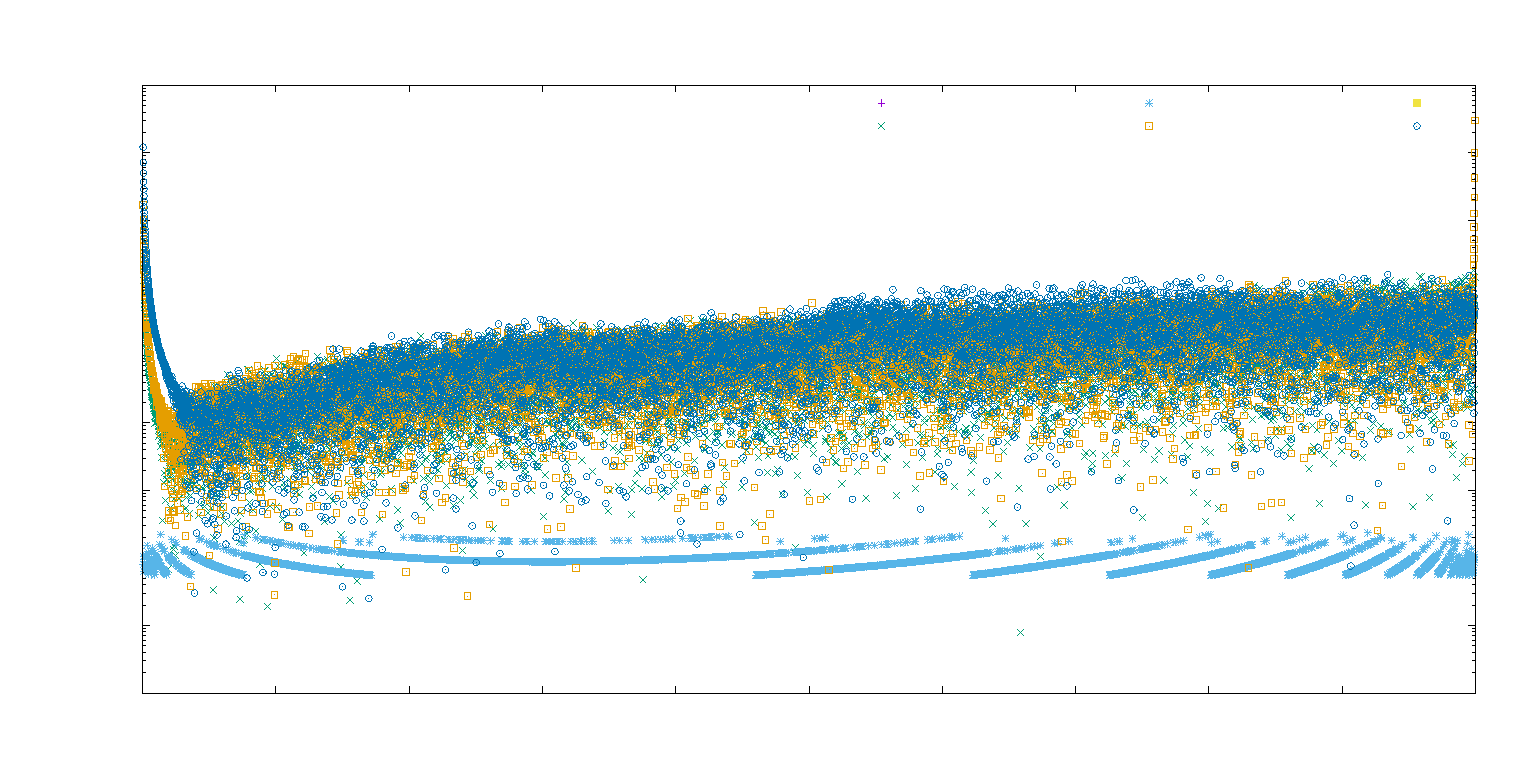
\includegraphics[width={720.00bp},height={360.00bp}]{./chapter2/graphs/phys_all_10K.eps}}%
    \gplfronttext
  \end{picture}%
\endgroup
}
	\caption[Residual in Lane-Emden polytrope code]{
	The residual for several numerical models of polytrope, as in \equref{RMSR}, following \equref{newtonian:static1}.
	\label{fig:chapter2:polyresid}}
\end{figure*}

\subsection{Scaling relations}\label{subsec:chapter2:code3}
\lipsum[1].  

\begin{figure}
	\resizebox{\linewidth}{!}{% GNUPLOT: LaTeX picture with Postscript
\begingroup
  \makeatletter
  \providecommand\color[2][]{%
    \GenericError{(gnuplot) \space\space\space\@spaces}{%
      Package color not loaded in conjunction with
      terminal option `colourtext'%
    }{See the gnuplot documentation for explanation.%
    }{Either use 'blacktext' in gnuplot or load the package
      color.sty in LaTeX.}%
    \renewcommand\color[2][]{}%
  }%
  \providecommand\includegraphics[2][]{%
    \GenericError{(gnuplot) \space\space\space\@spaces}{%
      Package graphicx or graphics not loaded%
    }{See the gnuplot documentation for explanation.%
    }{The gnuplot epslatex terminal needs graphicx.sty or graphics.sty.}%
    \renewcommand\includegraphics[2][]{}%
  }%
  \providecommand\rotatebox[2]{#2}%
  \@ifundefined{ifGPcolor}{%
    \newif\ifGPcolor
    \GPcolorfalse
  }{}%
  \@ifundefined{ifGPblacktext}{%
    \newif\ifGPblacktext
    \GPblacktexttrue
  }{}%
  % define a \g@addto@macro without @ in the name:
  \let\gplgaddtomacro\g@addto@macro
  % define empty templates for all commands taking text:
  \gdef\gplbacktext{}%
  \gdef\gplfronttext{}%
  \makeatother
  \ifGPblacktext
    % no textcolor at all
    \def\colorrgb#1{}%
    \def\colorgray#1{}%
  \else
    % gray or color?
    \ifGPcolor
      \def\colorrgb#1{\color[rgb]{#1}}%
      \def\colorgray#1{\color[gray]{#1}}%
      \expandafter\def\csname LTw\endcsname{\color{white}}%
      \expandafter\def\csname LTb\endcsname{\color{black}}%
      \expandafter\def\csname LTa\endcsname{\color{black}}%
      \expandafter\def\csname LT0\endcsname{\color[rgb]{1,0,0}}%
      \expandafter\def\csname LT1\endcsname{\color[rgb]{0,1,0}}%
      \expandafter\def\csname LT2\endcsname{\color[rgb]{0,0,1}}%
      \expandafter\def\csname LT3\endcsname{\color[rgb]{1,0,1}}%
      \expandafter\def\csname LT4\endcsname{\color[rgb]{0,1,1}}%
      \expandafter\def\csname LT5\endcsname{\color[rgb]{1,1,0}}%
      \expandafter\def\csname LT6\endcsname{\color[rgb]{0,0,0}}%
      \expandafter\def\csname LT7\endcsname{\color[rgb]{1,0.3,0}}%
      \expandafter\def\csname LT8\endcsname{\color[rgb]{0.5,0.5,0.5}}%
    \else
      % gray
      \def\colorrgb#1{\color{black}}%
      \def\colorgray#1{\color[gray]{#1}}%
      \expandafter\def\csname LTw\endcsname{\color{white}}%
      \expandafter\def\csname LTb\endcsname{\color{black}}%
      \expandafter\def\csname LTa\endcsname{\color{black}}%
      \expandafter\def\csname LT0\endcsname{\color{black}}%
      \expandafter\def\csname LT1\endcsname{\color{black}}%
      \expandafter\def\csname LT2\endcsname{\color{black}}%
      \expandafter\def\csname LT3\endcsname{\color{black}}%
      \expandafter\def\csname LT4\endcsname{\color{black}}%
      \expandafter\def\csname LT5\endcsname{\color{black}}%
      \expandafter\def\csname LT6\endcsname{\color{black}}%
      \expandafter\def\csname LT7\endcsname{\color{black}}%
      \expandafter\def\csname LT8\endcsname{\color{black}}%
    \fi
  \fi
    \setlength{\unitlength}{0.0500bp}%
    \ifx\gptboxheight\undefined%
      \newlength{\gptboxheight}%
      \newlength{\gptboxwidth}%
      \newsavebox{\gptboxtext}%
    \fi%
    \setlength{\fboxrule}{0.5pt}%
    \setlength{\fboxsep}{1pt}%
    \definecolor{tbcol}{rgb}{1,1,1}%
\begin{picture}(14400.00,7200.00)%
    \gplgaddtomacro\gplbacktext{%
      \csname LTb\endcsname%%
      \put(814,704){\makebox(0,0)[r]{\strut{}$2^{-7}$}}%
      \put(814,1093){\makebox(0,0)[r]{\strut{}$2^{-6}$}}%
      \put(814,1482){\makebox(0,0)[r]{\strut{}$2^{-5}$}}%
      \put(814,1871){\makebox(0,0)[r]{\strut{}$2^{-4}$}}%
      \put(814,2260){\makebox(0,0)[r]{\strut{}$2^{-3}$}}%
      \put(814,2649){\makebox(0,0)[r]{\strut{}$2^{-2}$}}%
      \put(814,3038){\makebox(0,0)[r]{\strut{}$2^{-1}$}}%
      \put(814,3427){\makebox(0,0)[r]{\strut{}$2^{0}$}}%
      \put(814,3816){\makebox(0,0)[r]{\strut{}$2^{1}$}}%
      \put(814,4205){\makebox(0,0)[r]{\strut{}$2^{2}$}}%
      \put(814,4594){\makebox(0,0)[r]{\strut{}$2^{3}$}}%
      \put(814,4983){\makebox(0,0)[r]{\strut{}$2^{4}$}}%
      \put(814,5372){\makebox(0,0)[r]{\strut{}$2^{5}$}}%
      \put(814,5761){\makebox(0,0)[r]{\strut{}$2^{6}$}}%
      \put(814,6150){\makebox(0,0)[r]{\strut{}$2^{7}$}}%
      \put(814,6539){\makebox(0,0)[r]{\strut{}$2^{8}$}}%
      \put(946,484){\makebox(0,0){\strut{}$0$}}%
      \put(3557,484){\makebox(0,0){\strut{}$0.2$}}%
      \put(6169,484){\makebox(0,0){\strut{}$0.4$}}%
      \put(8780,484){\makebox(0,0){\strut{}$0.6$}}%
      \put(11392,484){\makebox(0,0){\strut{}$0.8$}}%
      \put(14003,484){\makebox(0,0){\strut{}$1$}}%
    }%
    \gplgaddtomacro\gplfronttext{%
      \csname LTb\endcsname%%
      \put(209,3621){\rotatebox{-270}{\makebox(0,0){\large\strut{}$\abs{\theta_\mathrm{num}-\theta_\mathrm{exact}}_{N}/\abs{\theta_\mathrm{num}-\theta_\mathrm{exact}}_{2N}$}}}%
      \put(7474,154){\makebox(0,0){\large\strut{}$r/R$}}%
      \csname LTb\endcsname%%
      \put(13016,6366){\makebox(0,0)[r]{\strut{}$n=0.0$}}%
      \csname LTb\endcsname%%
      \put(13016,6146){\makebox(0,0)[r]{\strut{}$n=1.0$}}%
      \csname LTb\endcsname%%
      \put(13016,5926){\makebox(0,0)[r]{\strut{}$n=5.0$}}%
      \csname LTb\endcsname%%
      \put(7474,6869){\makebox(0,0){\Large\strut{}Scaling of Errors in Exact Polytropes, scale factor 2}}%
    }%
    \gplbacktext
    \put(0,0){\includegraphics[width={720.00bp},height={360.00bp}]{./chapter2/graphs/scale_all_exact.eps}}%
    \gplfronttext
  \end{picture}%
\endgroup
}
	\caption[Exact error scaling in polytrope code]{Error scaling for polytropes, compared to exact solutions.  The $n=1$ and $n=5$ polytrope errors scale like $2^4$ as expected. 
	\label{fig:chapter2:scalepolyexact}}
\end{figure}
\begin{figure}
	\resizebox{\linewidth}{!}{% GNUPLOT: LaTeX picture with Postscript
\begingroup
  \makeatletter
  \providecommand\color[2][]{%
    \GenericError{(gnuplot) \space\space\space\@spaces}{%
      Package color not loaded in conjunction with
      terminal option `colourtext'%
    }{See the gnuplot documentation for explanation.%
    }{Either use 'blacktext' in gnuplot or load the package
      color.sty in LaTeX.}%
    \renewcommand\color[2][]{}%
  }%
  \providecommand\includegraphics[2][]{%
    \GenericError{(gnuplot) \space\space\space\@spaces}{%
      Package graphicx or graphics not loaded%
    }{See the gnuplot documentation for explanation.%
    }{The gnuplot epslatex terminal needs graphicx.sty or graphics.sty.}%
    \renewcommand\includegraphics[2][]{}%
  }%
  \providecommand\rotatebox[2]{#2}%
  \@ifundefined{ifGPcolor}{%
    \newif\ifGPcolor
    \GPcolorfalse
  }{}%
  \@ifundefined{ifGPblacktext}{%
    \newif\ifGPblacktext
    \GPblacktexttrue
  }{}%
  % define a \g@addto@macro without @ in the name:
  \let\gplgaddtomacro\g@addto@macro
  % define empty templates for all commands taking text:
  \gdef\gplbacktext{}%
  \gdef\gplfronttext{}%
  \makeatother
  \ifGPblacktext
    % no textcolor at all
    \def\colorrgb#1{}%
    \def\colorgray#1{}%
  \else
    % gray or color?
    \ifGPcolor
      \def\colorrgb#1{\color[rgb]{#1}}%
      \def\colorgray#1{\color[gray]{#1}}%
      \expandafter\def\csname LTw\endcsname{\color{white}}%
      \expandafter\def\csname LTb\endcsname{\color{black}}%
      \expandafter\def\csname LTa\endcsname{\color{black}}%
      \expandafter\def\csname LT0\endcsname{\color[rgb]{1,0,0}}%
      \expandafter\def\csname LT1\endcsname{\color[rgb]{0,1,0}}%
      \expandafter\def\csname LT2\endcsname{\color[rgb]{0,0,1}}%
      \expandafter\def\csname LT3\endcsname{\color[rgb]{1,0,1}}%
      \expandafter\def\csname LT4\endcsname{\color[rgb]{0,1,1}}%
      \expandafter\def\csname LT5\endcsname{\color[rgb]{1,1,0}}%
      \expandafter\def\csname LT6\endcsname{\color[rgb]{0,0,0}}%
      \expandafter\def\csname LT7\endcsname{\color[rgb]{1,0.3,0}}%
      \expandafter\def\csname LT8\endcsname{\color[rgb]{0.5,0.5,0.5}}%
    \else
      % gray
      \def\colorrgb#1{\color{black}}%
      \def\colorgray#1{\color[gray]{#1}}%
      \expandafter\def\csname LTw\endcsname{\color{white}}%
      \expandafter\def\csname LTb\endcsname{\color{black}}%
      \expandafter\def\csname LTa\endcsname{\color{black}}%
      \expandafter\def\csname LT0\endcsname{\color{black}}%
      \expandafter\def\csname LT1\endcsname{\color{black}}%
      \expandafter\def\csname LT2\endcsname{\color{black}}%
      \expandafter\def\csname LT3\endcsname{\color{black}}%
      \expandafter\def\csname LT4\endcsname{\color{black}}%
      \expandafter\def\csname LT5\endcsname{\color{black}}%
      \expandafter\def\csname LT6\endcsname{\color{black}}%
      \expandafter\def\csname LT7\endcsname{\color{black}}%
      \expandafter\def\csname LT8\endcsname{\color{black}}%
    \fi
  \fi
    \setlength{\unitlength}{0.0500bp}%
    \ifx\gptboxheight\undefined%
      \newlength{\gptboxheight}%
      \newlength{\gptboxwidth}%
      \newsavebox{\gptboxtext}%
    \fi%
    \setlength{\fboxrule}{0.5pt}%
    \setlength{\fboxsep}{1pt}%
    \definecolor{tbcol}{rgb}{1,1,1}%
\begin{picture}(14400.00,7200.00)%
    \gplgaddtomacro\gplbacktext{%
      \csname LTb\endcsname%%
      \put(814,704){\makebox(0,0)[r]{\strut{}$2^{-2}$}}%
      \put(814,1288){\makebox(0,0)[r]{\strut{}$2^{-1}$}}%
      \put(814,1871){\makebox(0,0)[r]{\strut{}$2^{0}$}}%
      \put(814,2455){\makebox(0,0)[r]{\strut{}$2^{1}$}}%
      \put(814,3038){\makebox(0,0)[r]{\strut{}$2^{2}$}}%
      \put(814,3622){\makebox(0,0)[r]{\strut{}$2^{3}$}}%
      \put(814,4205){\makebox(0,0)[r]{\strut{}$2^{4}$}}%
      \put(814,4789){\makebox(0,0)[r]{\strut{}$2^{5}$}}%
      \put(814,5372){\makebox(0,0)[r]{\strut{}$2^{6}$}}%
      \put(814,5956){\makebox(0,0)[r]{\strut{}$2^{7}$}}%
      \put(814,6539){\makebox(0,0)[r]{\strut{}$2^{8}$}}%
      \put(946,484){\makebox(0,0){\strut{}$0$}}%
      \put(2252,484){\makebox(0,0){\strut{}$0.1$}}%
      \put(3557,484){\makebox(0,0){\strut{}$0.2$}}%
      \put(4863,484){\makebox(0,0){\strut{}$0.3$}}%
      \put(6169,484){\makebox(0,0){\strut{}$0.4$}}%
      \put(7475,484){\makebox(0,0){\strut{}$0.5$}}%
      \put(8780,484){\makebox(0,0){\strut{}$0.6$}}%
      \put(10086,484){\makebox(0,0){\strut{}$0.7$}}%
      \put(11392,484){\makebox(0,0){\strut{}$0.8$}}%
      \put(12697,484){\makebox(0,0){\strut{}$0.9$}}%
      \put(14003,484){\makebox(0,0){\strut{}$1$}}%
    }%
    \gplgaddtomacro\gplfronttext{%
      \csname LTb\endcsname%%
      \put(209,3621){\rotatebox{-270}{\makebox(0,0){\large\strut{}$\text{res}_{N}/\text{res}_{2N}$}}}%
      \put(7474,154){\makebox(0,0){\large\strut{}$r/R$}}%
      \csname LTb\endcsname%%
      \put(2794,2637){\makebox(0,0)[r]{\strut{}Euler $n=1.0$}}%
      \csname LTb\endcsname%%
      \put(2794,2417){\makebox(0,0)[r]{\strut{}Poisson $n=1.0$}}%
      \csname LTb\endcsname%%
      \put(2794,2197){\makebox(0,0)[r]{\strut{}Euler $n=1.5$}}%
      \csname LTb\endcsname%%
      \put(2794,1977){\makebox(0,0)[r]{\strut{}Poisson $n=1.5$}}%
      \csname LTb\endcsname%%
      \put(2794,1757){\makebox(0,0)[r]{\strut{}Euler $n=3.0$}}%
      \csname LTb\endcsname%%
      \put(2794,1537){\makebox(0,0)[r]{\strut{}Poisson $n=3.0$}}%
      \csname LTb\endcsname%%
      \put(7474,6869){\makebox(0,0){\Large\strut{}Scaling of Residuals in Background Equations, scale factor = 2}}%
    }%
    \gplbacktext
    \put(0,0){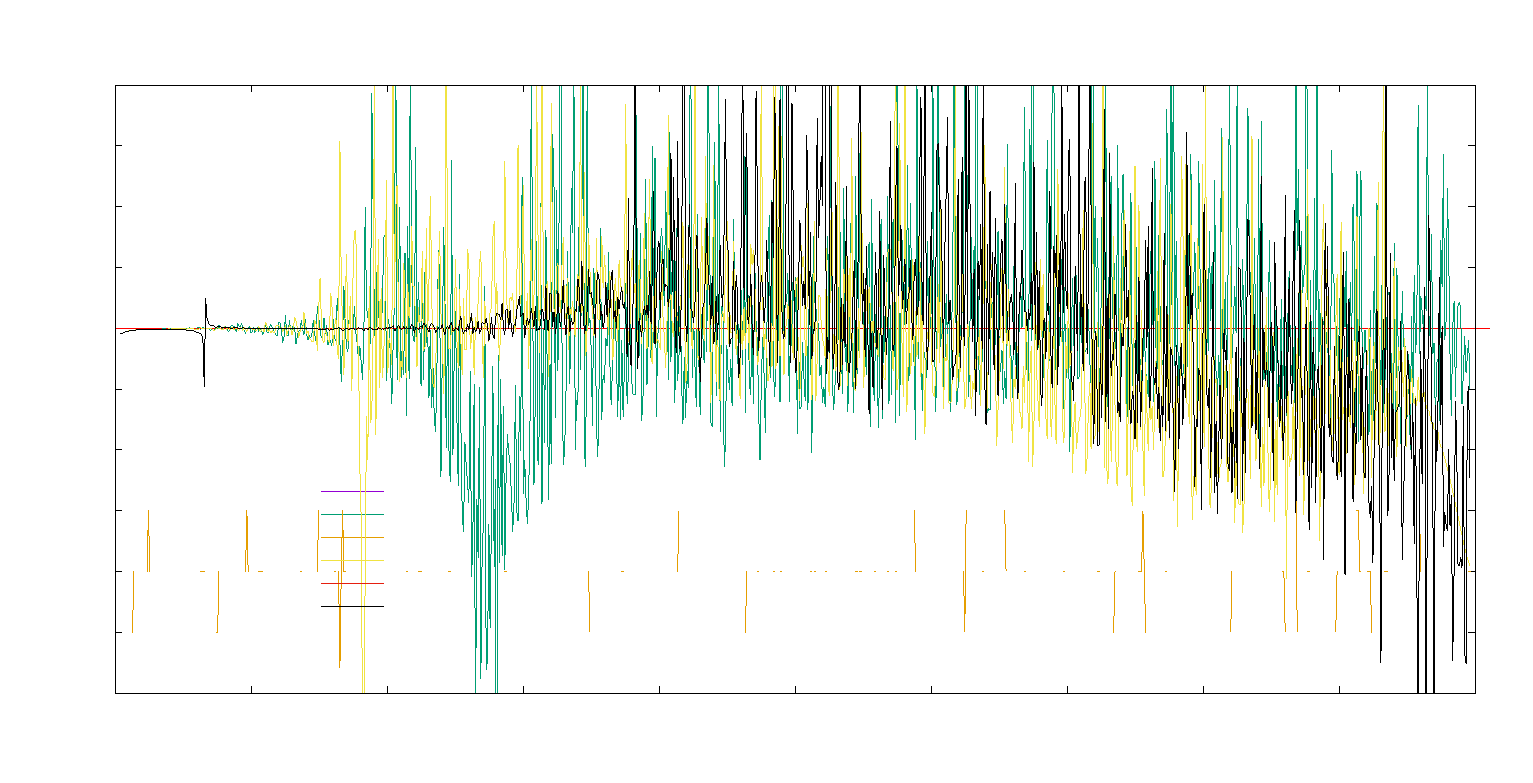
\includegraphics[width={720.00bp},height={360.00bp}]{./chapter2/graphs/scale_all_phys.eps}}%
    \gplfronttext
  \end{picture}%
\endgroup
}
	\caption[Residual scaling in polytrope code]{The residual scaling for several polytropes, with the residuals as in \equref{Residual}.  The scaling varies sharply, but strongly clusters around the $2^4$ line, as expected.\label{fig:chapter2:scalepolyresid}}
\end{figure}

\subsection{Normal mode calculation}\label{subsec:chapter2:code4}

\lipsum[2][1-5]
A schematic of this is shown in \figref{chapter2:innerouter}.

\begin{figure}[h]
\begin{center}
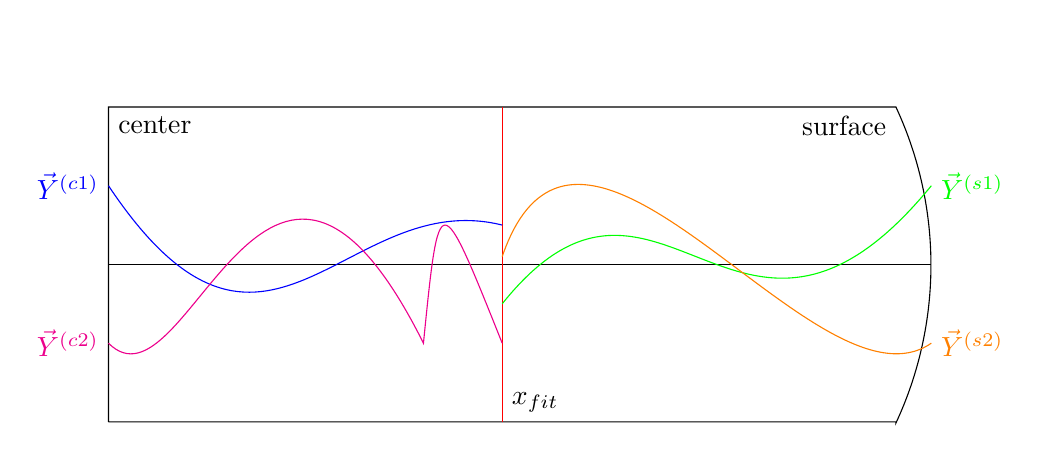
\begin{tikzpicture}
    \draw (0,2) -- (10.45,2);
    \draw (0,0) -- (0,4) -- (10,4) arc[start angle=25, end angle=-25, radius=4.75] -- (10,0) -- (0,0);
    \node[anchor=north west] at (0,4) {center};
    \node[anchor=north east] at (10,4) {surface};
    
    \draw[color=red] (5,0) -- (5,4);
    \node[anchor=south west] at (5,0) {$x_\text{fit}$};
    
    \draw[color=blue]    (0,3) .. controls (2,0) and (3,3) .. (5,2.5);
    \draw[color=magenta] (0,1) .. controls (1,0) and (2,5) .. (4,1) .. controls (4.2, 3) .. (5,1);
    \node[color=blue,    anchor=east] at (0,3) {${\vec{Y}}^{(c1)}$};
    \node[color=magenta, anchor=east] at (0,1) {${\vec{Y}}^{(c2)}$};
    
    \draw[color=green]  (10.45,3) .. controls (8,0) and (7, 4) .. (5, 1.5);
    \draw[color=orange] (10.45,1) .. controls (9,0) and (6, 5) .. (5, 2.1);
    \node[color=green,  anchor=west] at (10.45,3) {${\vec{Y}}^{(s1)}$};
    \node[color=orange, anchor=west] at (10.45,1) {${\vec{Y}}^{(s2)}$};
\end{tikzpicture}
\caption[Sketch of nonradial mode solution method]{
	A sketch of the solution process for nonradial modes.
	The two BCs at each boundary give the two solutions in each region, and the values of these four solutions at $x_\mathrm{fit}$ 
	are used in the Wronskian for find $\bar{\omega}$, then fit together to create the physical solution.
\label{fig:chapter2:innerouter}}
\end{center}
\end{figure}
%%%%%%%%%%%%%%%%%%%%%%%%%%%%%%%%%%%%%%%%
